Con il termine \emph{superficie estesa} ci si riferisce ad un solido soggetto a scambio termico per conduzione al proprio interno e per convezione attraverso il contorno. 
\begin{figure}
\centering
\psfrag{w}{$w$}
\psfrag{t}{$t$}
\psfrag{L}{$L$}
\psfrag{T0}{$T_0$}
\psfrag{hP}{$h_P$}
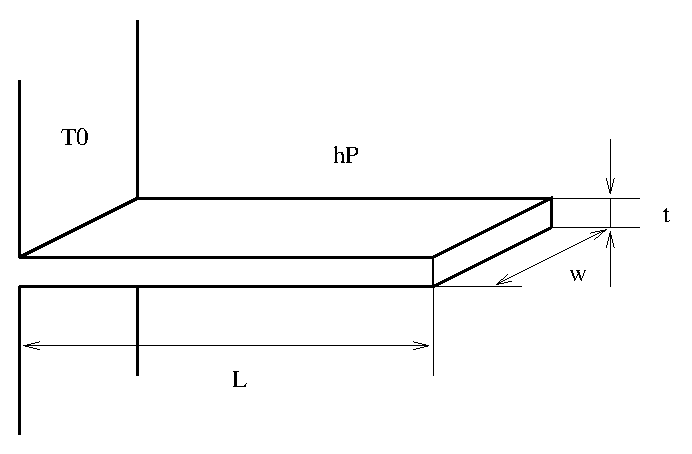
\includegraphics[width=0.5\textwidth]{./figures/eps/fin.eps}
\caption{Schema di un'aletta a base rettangolare e sezione costante.}
\label{fig:fin}
\end{figure}
Una superficie estesa utilizzata per migliorare lo scambio termico tra un solido ed il fluido che lo circonda \`e detta \emph{aletta} (si veda \figref{fig:fin}). Nel caso in cui il numero di Biot:
\begin{equation*}
\Biot \eqbydef \frac{h_P t w}{2 k \left( t + w \right)}
\end{equation*}
sia sufficientemente piccolo (tipicamente inferiore a $0.1$), si pu\`o assumere che la temperatura sia uniforme sulla sezione trasversale dell'aletta. Supponendo che la temperatura asintotica del fluido che lambisce l'aletta $T_{\infty}$ sia costante, il profilo di temperatura nella direzione longitudinale \`e fornito dall'equazione del calore monodimensionale:
\begin{equation}
-\frac{\ud^2 \theta}{\ud x^2} + a\theta = 0,\quad 0<x<L,
\label{eq:heat}
\end{equation}
ove si \`e posto $\theta\eqbydef T - T_{\infty}$ e $a \eqbydef 2h_P \left( w + t\right) / kwt$. Per fissare le condizioni al bordo, si assuma che la base dell'aletta sia alla temperatura della superficie $T_0$ e che non vi sia scambio di calore attraverso l'altra estremit\`a (condizione di \emph{punta adiabatica}):
\begin{equation*}
\function{\theta}{0} = T_0 - T_{\infty},\quad %
\function{\frac{\ud\theta}{\ud x}}{L} = 0.
\end{equation*}
Per maggiori dettagli si veda \cite{Incropera.DeWitt:1996}

Una soluzione approssimata dell'equazione precedente pu\`o essere ottenuta discretizzandola secondo il metodo delle differenze finite. Introduciamo una partizione uniforme $\Th$ dell'intervallo $\openint{0}{L}$ in $M$ elementi e consideriamo l'interpolante della soluzione ai nodi $x_j = jh$, $j=0,\ldots,M$, essendo $h\eqbydef L / M$ il passo di griglia. Indichiamo, inoltre, con $u_i=u_h(x_i)$, $i=0,\ldots,M$ i valori nodali della soluzione approssimata, che costituiscono le incognite del problema. Per le condizioni al bordo si ha che $u_0=\theta_0\eqbydef T_0 - T_{\infty}$. Si ottiene il seguente sistema lineare:
\begin{equation}
\label{eq:stfem}
A\mathbf{u}=\mathbf{b},
\end{equation}
essendo:
\begin{equation*}
\U=\left[u_0,\ldots,u_M\right]^T,\quad \mathbf{b}=\left[\theta_0,0,\ldots,0\right]^T,
\end{equation*}
e:
\begin{equation*}
\mathbb{R}^{(M+1)\times (M+1)}\ni A\eqbydef\left[
\begin{array}{ccccccc}
1       & 0         & 0         & \ldots    & 0         & 0     \\
-1      & 2+h^2 a   & -1        & \ldots    & 0         & 0     \\
\vdots  &           & \ddots    &           &           &       \\
0       & 0         & \ldots    & -1        & 2+h^2 a   & -1    \\
0       & 0         & \ldots    & 0         & -2        & 2+h^2 a     \\
\end{array}
\right].
\end{equation*}

La matrice $A$ \`e a dominanza diagonale stretta per righe. Il problema
discreto pu\`o, quindi, essere risolto mediante  il metodo di
Gauss-Seidel (si veda \cite[\extref{4.2}]{Quarteroni.Sacco.ea:2000}
). Si verifica facilmente che la $(k+1)$-esima iterazione di Gauss-Seidel per il caso in esame si scrive:
\begin{equation*}
u _i\iter{k+1}=\frac{u\iter{k+1}_{i-1} + u\iter{k}_{i+1}}{2 + h^2 a},\quad i=1,\ldots,M-1
\end{equation*}
e:
\begin{equation*}
u_0\iter{k+1} = \theta_0,\quad u _M\iter{k+1}=\frac{2}{2+h^2 a}u\iter{k+1}_{M-1}.
\end{equation*}
Si assume raggiunta la convergenza quando la norma euclidea della differenza tra due iterate successive \`e inferiore ad una fissata tolleranza $\tau$:
\begin{equation*}
\norm{ \U\iter{k+1} - \U\iter{k} }\le\tau.
\end{equation*}

Una possibile implementazione in linguaggio C++ del metodo proposto \`e la
seguente:
\lstset{basicstyle=\scriptsize\sf}
\lstinputlisting{./es/fin.cpp}
\lstset{basicstyle=\sf}

Oltre ai costrutti base comuni ai linguaggi di programmazione di alto
livello, il C++ offre una collezione di librerie standard che
implementano funzioni, classi, costanti ed oggetti di uso
frequente. Nel caso in esame sono state utilizzate le librerie
seguenti: \emph{iostream}, che implementa le classi per l'I/O sui
canali standard in ingresso ed uscita (\cpp{std::cin} e
\cpp{std::cout}); \emph{fstream}, che implementa le classi per
l'I/O su \emph{file}; \emph{cmath.h}, in cui sono definite le funzioni
matematiche di uso comune; \emph{vector}, che contiene
l'implementazione di un \cpp{template} \cpp{vector} per la
gestione degli \emph{array}. Si noti che la direttiva \cpp{using
namespace} \cpp{std} consente di accedere ai nomi del \cpp{namespace}
\cpp{std} omettendo la risoluzione esplicita, ovvero di scrivere
semplicemente \cpp{cout} in luogo di \cpp{std::cout}.

Le variabili globali sono state definite all'esterno del \emph{main
program}, in modo da essere visibili ovunque all'interno del
\emph{file}. L'attributo \cpp{const} indica al compilatore che la
variabile non pu\`o trovarsi al primo membro di un'assegnazione. Se
introducessimo l'istruzione: 
\lstset{basicstyle=\scriptsize\sf}
\begin{lstlisting}
const int MMAX = 501;
...
int main(){     
    MMAX = 30;
    ...
}
\end{lstlisting}
\lstset{basicstyle=\sf}
e tentassimo di compilare otterremmo il seguente messaggio d'errore:
\begin{verbatim}
fin.cpp: In function `int main()':
fin.cpp:44: error: assignment of read-only variable `MMAX'
\end{verbatim}
Lo stile dei commenti \`e conforme alla sintassi di Doxygen, un
\emph{software} per la generazione automatica della documentazione, di
cui si discuter\`a in un'esercitazione successiva.

All'inizio del programma viene richiesto all'utente di inserire il
numero $M$ di elementi della discretizzazione. \`E stato inserito un
semplice meccanismo di controllo che ripete la richiesta qualora il
numero di elementi sia inferiore a $1$ o superiore a $MMAX$. Tale
controllo \`e implementato mediante un ciclo con controllo in coda
\cpp{do ... while}.

L'elemento finito corrispondente alla soluzione approssimata viene
definito come un vettore di \cpp{double} mediante l'istruzione:
\lstset{basicstyle=\scriptsize\sf}
\begin{lstlisting}
vector<double> uh(M + 1);
\end{lstlisting}
\lstset{basicstyle=\sf}
che alloca lo spazio per $M+1$ elementi. La ragione per cui il tipo
degli elementi memorizzati nel vettore \`e dichiarato tra parentesi
angolari diverr\`a chiara quando verr\`a introdotto il concetto di
\cpp{template}. Per inizializzare il vettore si \`e utilizzato un
ciclo \cpp{for} in cui si accede agli elementi mediante
l'\cpp{operator[]} (\emph{accesso per indice}).

Verso la fine il codice proposto confronta la soluzione approssimata
con quella esatta:
\begin{equation*}
\function{\theta}{x} = \theta_0\frac{\function{\cosh}{\sqrt{a}\left(L - x\right)}}{\function{\cosh}{\sqrt{a}L}},
\end{equation*} e stima la norma $L^\infty$ dell'errore.

La scrittura su \emph{file} dei risultati sfrutta la class
\emph{ostream} e l'operatore di scorrimento \cpp{<<}.
L'istruzione
\lstset{basicstyle=\scriptsize\sf}
\begin{lstlisting}
f.close();
\end{lstlisting}
\lstset{basicstyle=\sf}
chiude il canale di accesso al \emph{file}. 

Utilizzando i valori dei parametri riportati in \tabref{tab:parameters} e 
discretizzando con $M=20$ elementi, si ottiene la soluzione approssimata
rappresentata in \figref{fig:fin:results}. Insieme alla soluzione approssimata
\`e stata disegnata anche la soluzione esatta (con tratto continuo).
%
\begin{figure}
\subfigure[Profilo di temperatura.]{
\psfrag{T}{$T$ ($\uK$)}
\psfrag{x}{$x$}
\psfrag{uh}{$u_h$}
\psfrag{u}{$\theta$}
\includegraphics[height=0.45\textwidth,angle=-90]{./figures/eps/fin.profile.eps}
}
\subfigure[Convergenza.]{
\psfrag{linf}{$\norm{ e }_{\hilbertL{\infty}{\Omega}}$}
\includegraphics[height=0.45\textwidth,angle=-90]{./figures/eps/fin.convergence.eps}
}
\caption{Soluzione approssimata ed esatta del problema definito dai
dati in \tabref{tab:parameters} e risultati sperimentali di convergenza.}
\label{fig:fin:results}
\end{figure}

\begin{table}
\centering
\begin{tabular}{|c|c|c|}
\hline
$k$     & $5$   & $\uW / (\um\uK)$ \\
\hline
$h_P$   & $10$  & $\uW / (\um^2\uK)$ \\
\hline
$L$     & $100$ & $\umm$ \\
\hline
$w$     & $50$  &  $\umm$ \\
\hline
$t$     & $5$   & $\umm$ \\
\hline
\end{tabular}
\caption{Parametri per la validazione del codice.}
\label{tab:parameters}
\end{table}

Si modifichi il programma proposto, in modo che risolva il sistema tridiagonale
con l'algoritmo di Thomas: si consideri la generica matrice $A \in \mathbb R^{n
\times n}$ non singolare e {\it tridiagonale}:
      \[
       A = \left [ \begin{array}{ccccc}
                  a_1 & c_1 & & & \\
                    e_1  & a_2 & c_2 &  & \\
                    & \ddots& \ddots & \ddots & \\
                     & & e_{n-2}& a_{n-1} & c_{n-1} \\
                    & &  & e_{n-1} & a_n \\ 
                  \end{array}
           \right ] .        
      \]
      Le matrici $L$ ed $U$ della corrispondente fattorizzazione 
      $LU$ sono matrici bidiagonali della forma:
      \[
      L = \left [ \begin{array}{ccccc}
                  1 & & & & \\
                  \delta_{1}& 1 & & & \\
                    & \ddots & \ddots & & \\
                    & & \delta_{n-2} & 1 & \\
                    & & & \delta_{n-1} & 1 \\ 
                  \end{array}
           \right ],               
       \qquad      \quad
        U = \left [ \begin{array}{ccccc}
                  \alpha_1 & c_1 & & & \\
                      & \alpha_2 & c_2 &  & \\
                    & & \ddots & \ddots & \\
                     & & & \alpha_{n-1} & c_{n-1} \\
                    & &  &  & \alpha_n \\ 
                  \end{array}
           \right ] ,        
      \]
      i cui coefficienti sono dati dalle seguenti relazioni 
      (\emph{algoritmo di Thomas}):
      \[
       \alpha_1=a_1,\qquad \delta_{i-1}=\frac{e_{i-1}}{\alpha_{i-1}}, 
         \qquad \alpha_i=a_i-\delta_{i-1} c_{i-1}, \qquad i=2,\ldots,n.
       \]

Si suggerisce di provare a scrivere una funzione, al posto di limitarsi a
sostituire le righe di codice opportune:

\lstset{basicstyle=\scriptsize\sf}
\begin{lstlisting}
  bool Thomas_solver(const std::vector<double>& d1, const std::vector<double>& d2, 
                     const std::vector<double>& d3, const std::vector<double>& b, 
                     std::vector<double>& uh)
\end{lstlisting}
\lstset{basicstyle=\sf}

dove \cpp{d1}, \cpp{d2}, \cpp{d3} sono vettori contenenti le diagonali 
non nulle della matrice $A$, \cpp{uh} \`e il vettore soluzione. La funzione
restituisce un valore booleano che assume valore \cpp{true} se il solutore ha 
terminato regolarmente l'esecuzione e \cpp{false} in caso contrario (valore pivotale zero).  
 
Il testo di questa esercitazione \`e ispirato ad un esercizio proposto in \cite{Hecht.Danalia.ea:2003}.
